\documentclass[../notes.tex]{subfiles}

\pagestyle{main}
\renewcommand{\chaptermark}[1]{\markboth{\chaptername\ \thechapter\ (#1)}{}}
\setcounter{chapter}{4}

\begin{document}




\chapter{Applications and Generalizations}
\section{Special Normal Subgroups}
\begin{itemize}
    \item \marginnote{10/24:}Last time: If $H\triangleleft S_n$, $n\neq 4$, then $H=\{e\},S_n,A_n$. If $n=4$, $H$ can also equal $\{e\}\cup\{(xx)(xx)\}$.
    \item Theorem: Let $n\neq 4$. Then the only normal subgroups of $A_n$ are the identity and $A_n$.
    \begin{itemize}
        \item Let $H\triangleleft A_n\triangleleft S_n$. From this, you could propose concluding that since we know all normal subgroups of $S_n$, and $H$ is less than or equal to $A_n$, we know that $H=\{e\},A_n$.
        \item Issue: $\triangleleft$ is not transitive. Conjugacy classes change depending on where you're sitting.
        \item Consider $A,B,C$: If $A\triangleleft B\triangleleft C$, then is $A\triangleleft C$?
        \item This theorem is on HW5.
        \item Counterexample:
        \begin{align*}
            A &= \gen{(1,2)(3,4)}&
            B &= \{e\}\cup\{(xx)(xx)\}&
            C &= S_4
        \end{align*}
        \begin{itemize}
            \item This is not so far from the simplest example.
        \end{itemize}
        \item Calegari reemphasizes that, "if you understand everything about $S_4$, then you understand everything in this class."
    \end{itemize}
    \item We know that if $H\leq A_4$, then $|H|\big|12$ by Lagrange's theorem.
    \item Claim: $A_4$ has no subgroups of order 6.
    \begin{itemize}
        \item If $H$ has index 2, then $H\triangleleft A_4$. This was a HW problem.
        \item Thus, we can try to understand conjugacy classes in $A_n$. Whereas in $S_n$, we have a beautifully simple way to characterize all conjugacy classes, we do not have that in $A_n$. For example, $(1,2,3)$ and $(1,3,2)$ are not conjugate. $(2,3)(1,2,3)(2,3)=(1,3,2)$. $(1,2)(1,2,3)(1,2)=(2,1,3)$. $(1,3)(1,2,3)(1,3)=(3,2,1)$. But none of these transpositions are in $A_n$.
        \item There are four conjugacy classes in $A_4$.
        \begin{align*}
            \{e\}&&
            \{(12)(34),(13)(24),(14)(23)\}&&
            \{(123),(243),(134),(142)\}&&
            \{(132),(234),(143),(124)\}
        \end{align*}
        \begin{itemize}
            \item Note that if $x,y\in A_4$ are of order 3, either $x\sim y$ or $x\sim y^{-1}$.
        \end{itemize}
        \item In $A_5$, all 3-cycles are conjugate; in $A_4$, they're not.
        \item The sizes of the conjugacy classes in $A_4$ are $1+4+4+3$. That's enough to prove that there is no subgroup of order 6.
        \item Alternate proof.
        \begin{proof}
            Suppose for the sake of contradiction that $A_4$ has a normal subgroup $H$ of index 2. Then by the proposition from Lecture 4.1, there exists a surjective homomorphism from $A_4\to A_4/H$. Additionally, since $|A_4/H|=2$ and there is only one group of order 2, $A_4/H\cong\Z/2\Z$. Thus, there exists a surjective homomorphism $\phi:A_4\to\Z/2\Z$.\par
            We know that every alternating group (including $A_4$) is generated by 3-cycles. Let $\sigma$ be an arbitrary 3-cycle generator of $A_4$. We know that $\phi(\sigma)=0$ or $\phi(\sigma)=1$. If $\phi(\sigma)=1$, then
            \begin{equation*}
                0 = \phi(e) = \phi(\sigma^3) = 3\phi(\sigma) = 1+_21+_21 = 1
            \end{equation*}
            which clearly cannot happen. Thus, $\phi(\sigma)=0$. Consequently, the image of all of the generators of $A_4$ under $\phi$ is 0. But this implies that $\phi(A_4)=\{0\}\subsetneq\Z/2\Z$, contradicting our hypothesis that $\phi$ is surjective.
        \end{proof}
    \end{itemize}
    \item Here ends the material that will be covered on the midterm.
    \item We now move on to something we will come back to later.
    \item $A_n$ in nature for $n=4,5$.
    \begin{figure}[h!]
        \centering
        \begin{subfigure}[b]{0.19\linewidth}
            \centering
            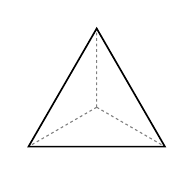
\begin{tikzpicture}
                \draw [gray,dash pattern=on 1pt off 1pt]
                    (0,0) -- (90:1)
                    (0,0) -- (-150:1)
                    (0,0) -- (-30:1)
                ;
                \draw [semithick] (90:1) -- (-150:1) -- (-30:1) -- cycle;
            \end{tikzpicture}
            \vspace{2.5mm}
            \caption{Tetrahedron.}
            \label{fig:platonicSolidsa}
        \end{subfigure}
        \begin{subfigure}[b]{0.19\linewidth}
            \centering
            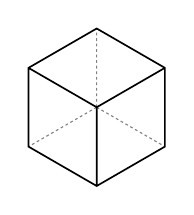
\begin{tikzpicture}
                \draw [gray,dash pattern=on 1pt off 1pt]
                    (0,0) -- (90:1)
                    (0,0) -- (-150:1)
                    (0,0) -- (-30:1)
                ;
                \draw [semithick]
                    (30:1) \foreach \i in {90,150,...,330} {-- (\i:1)} -- cycle
                    (0,0) -- (30:1)
                    (0,0) -- (150:1)
                    (0,0) -- (-90:1)
                ;
            \end{tikzpicture}
            \caption{Cube.}
            \label{fig:platonicSolidsb}
        \end{subfigure}
        \begin{subfigure}[b]{0.19\linewidth}
            \centering
            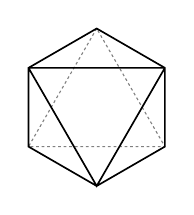
\begin{tikzpicture}[miter limit=2]
                \draw [gray,dash pattern=on 1pt off 1pt] (90:1) -- (-150:1) -- (-30:1) -- cycle;
                \draw [semithick]
                    (30:1) \foreach \i in {90,150,...,330} {-- (\i:1)} -- cycle
                    (30:1) -- (150:1) -- (-90:1) -- cycle
                ;
            \end{tikzpicture}
            \caption{Octahedron.}
            \label{fig:platonicSolidsc}
        \end{subfigure}
        \begin{subfigure}[b]{0.19\linewidth}
            \centering
            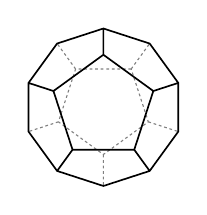
\begin{tikzpicture}
                \draw [gray,dash pattern=on 1pt off 1pt]
                    (54:0.6) \foreach \i in {126,198,...,342} {-- (\i:0.6)} -- cycle
                    \foreach \i in {54,126,...,342} {(\i:0.6) -- (\i:1)}
                ;
                \draw [semithick]
                    (18:{2/3}) \foreach \i in {90,162,...,306} {-- (\i:{2/3})} -- cycle
                    (18:1) \foreach \i in {54,90,...,342} {-- (\i:1)} -- cycle
                    \foreach \i in {18,90,...,306} {(\i:{2/3}) -- (\i:1)}
                ;
            \end{tikzpicture}
            \caption{Dodecahedron.}
            \label{fig:platonicSolidsd}
        \end{subfigure}
        \begin{subfigure}[b]{0.19\linewidth}
            \centering
            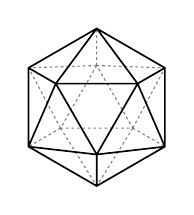
\begin{tikzpicture}
                \draw [gray,dash pattern=on 1pt off 1pt]
                    (90:0.53) -- (210:0.53) -- (330:0.53) -- cycle
                    \foreach \i in {30,90,150} {(90:0.53) -- (\i:1)}
                    \foreach \i in {150,210,270} {(210:0.53) -- (\i:1)}
                    \foreach \i in {270,330,30} {(330:0.53) -- (\i:1)}
                ;
                \draw [semithick]
                    (30:1) \foreach \i in {90,150,...,330} {-- (\i:1)} -- cycle
                    (30:0.6) -- (150:0.6) -- (-90:0.6) -- cycle
                    \foreach \i in {330,30,90} {(30:0.6) -- (\i:1)}
                    \foreach \i in {90,150,210} {(150:0.6) -- (\i:1)}
                    \foreach \i in {210,270,330} {(-90:0.6) -- (\i:1)}
                ;
            \end{tikzpicture}
            \caption{Icosahedron.}
            \label{fig:platonicSolidse}
        \end{subfigure}
        \caption{The platonic solids.}
        \label{fig:platonicSolids}
    \end{figure}
    \begin{itemize}
        \item Recall the cube group $\text{Cu}$.
        \item The cube is an example of a \textbf{platonic solid}.
        \item Other examples: Tetrahedron, octahedron, icosahedron, and dodecahedron. We define corresponding symmetry groups $\text{Te}$, $\text{Oc}$, $\text{Do}$, and $\text{Ic}$.
        \item Consider the tetrahedral group to start.
        \begin{itemize}
            \item Since any rigid motion permutes the vertices, we have a map $\text{Te}\hookrightarrow S_4$. Moving 2 vertices fixes the rest. Thus, $\text{Te}\leq S_4$. Therefore, $|\text{Te}|=12$ so $\text{Te}\cong A_4$.
        \end{itemize}
        \item We determined in HW2 that\dots
        \begin{itemize}
            \item $\text{Do}\hookrightarrow S_5$ and $|\text{Do}|=60$. Thus, $\text{Do}\cong A_5$.
        \end{itemize}
        \item Consider the octahedron.
        \begin{figure}[h!]
            \centering
            \begin{tikzpicture}[miter limit=2]
                \begin{scope}[scale=0.75,rotate=60]
                    \draw [rex!50!gray,very thin,dash pattern=on 1pt off 1pt]
                        (0,0) -- (90:1)
                        (0,0) -- (-150:1)
                        (0,0) -- (-30:1)
                    ;
                    \draw [rex]
                        (30:1) \foreach \i in {90,150,...,330} {-- (\i:1)} -- cycle
                        (0,0) -- (30:1)
                        (0,0) -- (150:1)
                        (0,0) -- (-90:1)
                    ;
                \end{scope}
        
                \draw [gray,dash pattern=on 1pt off 1pt] (90:1) -- (-150:1) -- (-30:1) -- cycle;
                \draw [semithick]
                    (30:1) \foreach \i in {90,150,...,330} {-- (\i:1)} -- cycle
                    (30:1) -- (150:1) -- (-90:1) -- cycle
                ;
            \end{tikzpicture}
            \caption{Inscribing a cube in an octahedron.}
            \label{fig:CuOh}
        \end{figure}
        \begin{itemize}
            \item $|\text{Oc}|=6\cdot 4=24$. Rationale: Fix one vertex anywhere and then fix another (the other one can only take on the four adjacent positions, though); the positions of the rest are determined from these two.
            \item Let's look at fixing opposite faces. This does give an injective map to $S_4$, and it follows that $\text{Oc}\cong S_4$.
            \item Relation between $\text{Oc}$ and $\text{Cu}$. We can inscribe a cube in the octahedron by connecting each vertex of the cube to the midpoint of one of the faces of the octahedron and vice versa. Thus, we get maps $\text{Oc}\to\text{Cu}$, leading to $\text{Oc}\cong\text{Cu}$.
        \end{itemize}
        \item We can similarly inscribe a dodecahedron in an icosahedron.
        \item Thus, the cube and the octahedron have the same symmetry, and the dodecahedron and icosahedron have the same symmetry.
    \end{itemize}
    \item \textbf{Platonic solid}: A solid geometric shape in three dimensions for which the faces, edges, and vertices are all indistinguishable.
    \begin{itemize}
        \item We will study the platonic solids in more depth later.
    \end{itemize}
    \item Problem: What symmetries can objects in $\R^3$ have?
    \begin{itemize}
        \item Rephrase: What are the finite subgroups of $\text{SO}(3)$?
        \item An octagon is Calegari's favorite polygon.
        \item An octagonal prism has much the same symmetry in $\R^3$ as an octagon does in $\R^2$. This leads to $D_{2n}\leq\text{SO}(3)$.
        \begin{itemize}
            \item Recall the map from the blog post.
        \end{itemize}
        \item We also have $\Z/n\Z\leq D_{2n}$.
    \end{itemize}
    \item It follows that the groups $\Z/n\Z$, $D_{2n}$, $A_4$, $S_4$, and $S_5$ occur as finite subgroups of $\text{SO}(3)$.
    \item Theorem: All finite subgroups of $\text{SO}(3)$ are on this list. Moreover, all related versions are conjugate.
    \begin{itemize}
        \item This is a companion theorem to the theorem that there are only five platonic solids.
        \item Neither theorem implies the other, but they are related.
    \end{itemize}
    \item Infinite subgroups of $\text{SO}(3)$: $\text{O}(2)$, $\text{SO}(3)$, $\text{SO}(2)$.
    \item This theorem will be completely evident by the end of the course.
    \item You can either use this theorem to understand $A_4,A_5$, or use an understanding of $A_4,A_5$ to rationalize this theorem.
    \item Points to the main focus of the class: Understanding groups not just based on writing down elements but by their action on a certain set. This is the focus of the second half of the course.
    \item Midterm: 50 mins, closed book, Wednesday. Final exam must be in-person by department rules, but Calegari is fighting for us. Calegari is hoping that the midterm should not be a speed test.
    \begin{itemize}
        \item Trying to test our skills, not our ability to memorize stuff.
        \item How to do well: Learn group theory.
    \end{itemize}
    \item The quaternion group.
    \begin{itemize}
        \item A 4D vector space where you define a noncommutative product. If you just take 8 specific quaternions, the group of order 8 is distinct from $D_8$ but related.
    \end{itemize}
\end{itemize}



\section{Group Actions}
\begin{itemize}
    \item \marginnote{10/28:}Let $G$ be a group and $X$ be a set.
    \item \textbf{Group action} (of $G$ on $X$): A map $\cdot:G\times X\to X$ satisfying the following. \emph{Denoted by} $\bm{G\,\pmb{\acts}\,X}$.
    \begin{enumerate}
        \item For all $g,h\in G$ and $x\in X$, $g\cdot(h\cdot x)=gh\cdot x$.
        \item For all $x\in X$, $e\cdot x=x$.
    \end{enumerate}
    \item Note that condition 2 does not follow from condition 1, and an "inverse condition" follows from both.
    \begin{itemize}
        \item In particular, condition 1 relates certain elements of the domain of the group action but does not relate any elements of the domain to elements of $X$ (as condition 2 does).
        \item The inverse condition $g^{-1}\cdot(g\cdot x)=g\cdot(g^{-1}\cdot x)=x$ follows from conditions 1-2 via
        \begin{equation*}
            g^{-1}\cdot(g\cdot x) = g^{-1}g\cdot x
            = e\cdot x
            = x
            = e\cdot x
            = gg^{-1}\cdot x
            = g\cdot(g^{-1}\cdot x)
        \end{equation*}
    \end{itemize}
    \item Example: If $G$ is any group and $X$ is any set, we may define a group action by $g\cdot x=x$ for all $g\in G$ and $x\in X$.
    \item Lemma: Let $G\acts X$ and $g\in G$. Define $\psi_g:X\to X$ by $x\mapsto g\cdot x$. Then $\psi_g$ is a bijection.
    \begin{proof}
        Injectivity:
        \begin{align*}
            \psi_g(x) &= \psi_g(y)\\
            g\cdot x &= g\cdot y\\
            g^{-1}\cdot(g\cdot x) &= g^{-1}\cdot(g\cdot y)\\
            e\cdot x &= e\cdot y\\
            x &= y
        \end{align*}
        Surjectivity: Given $x\in X$, we want $y$ such that $\psi_g(y)=x$. Choose $y=g^{-1}\cdot x$.
    \end{proof}
    \item This allows us to recast group actions into the following equivalent form.
    \item Let $X$ be a set and $S_X$ be the set of all bijections from $X\to X$ under composition. Note that if $|X|=n$, then $S_X\cong S_n$.
    \item Proposition: An action $G$ on the set $X$ is equivalent to a homomorphism from $G$ to $S_X$ defined by $g\mapsto\psi_g$.
    \begin{proof}
        % WTS: $\psi_g\circ\psi_h=\psi_{gh}$. This would follow if $[\psi_g\circ\psi_h](x)=\psi_{gh}(x)$ for all $x\in X$. This would follow if $g\cdot(h\cdot x)=gh\cdot x$ for all $x\in X$. But we have this by the definition of a group action, as desired.\par
        % Conversely, given the described homomorphism, we have $g\cdot x=\psi_g(x)$. Thus,
        % \begin{equation*}
        %     g\cdot h\cdot x = g\cdot\psi_h(x) = [\psi_g\circ\psi_h](x) = \psi_{gh}(x) = gh\cdot x
        % \end{equation*}
        % and
        % \begin{equation*}
        %     e\cdot x = \psi_e(x) = x
        % \end{equation*}


        A statement of the proposition that makes it more clear what exactly it is we want to prove is, "there exists an action $\cdot:G\times X\to X$ iff there exists a homomorphism $\phi:G\to X$ defined by $g\mapsto\psi_g$." Let's begin.\par\smallskip
        Suppose first that $\cdot:G\times X\to X$ is group action of $G$ on $X$. Define $\phi:G\to S_X$ by $g\mapsto\psi_g$. To prove that $\phi$ is a homomorphism, it will suffice to show that $\phi(gh)=\phi(g)\circ\phi(h)$ for all $g,h\in G$. Let $g,h\in G$ be arbitrary. Then by condition 1, we have for any and all $x\in X$ that
        \begin{align*}
            g\cdot(h\cdot x) &= gh\cdot x\\
            \psi_g(\psi_h(x)) &= \psi_{gh}(x)\\
            [\psi_g\circ\psi_h](x) &= \psi_{gh}(x)\\
            [\phi(g)\circ\phi(h)](x) &= [\phi(gh)](x)
        \end{align*}
        Therefore, $\phi(gh)=\phi(g)\circ\phi(h)$, as desired.\par
        Now suppose that $\phi:G\to S_X$ is a homomorphism defined by $g\mapsto\psi_g$. Define $\cdot:G\times X\to X$ by $g\cdot x=[\phi(g)](x)$. To prove that $\cdot$ is a group action, it will suffice to show that for all $g,h\in G$ and $x\in X$, $g\cdot(h\cdot x)=gh\cdot x$ and $e\cdot x=x$. Let $g,h\in G$ and $x\in X$ be arbitrary. Then
        \begin{equation*}
            g\cdot(h\cdot x) = g\cdot\psi_h(x)
            = [\psi_g\circ\psi_h](x)
            = [\phi(g)\circ\phi(h)](x)
            = [\phi(gh)](x)
            = \psi_{gh}(x)
            = gh\cdot x
        \end{equation*}
        and
        \begin{equation*}
            e\cdot x = \psi_e(x) = x
        \end{equation*}
        as desired.
    \end{proof}
    \item You need to be careful with what the set is and what the group is; $x\cdot y$ probably doesn't make any sense (unless you start to get into cases where $X$ is a group, too).
    \item \textbf{Kernel} (of a group action): The set of all $g\in G$ such that $g\cdot x=x$ for all $x\in X$.
    \begin{itemize}
        \item The kernel is a (normal) subgroup of $G$.
        \item We know this since it is equivalent to the kernel of the homomorphism described by the above proposition.
    \end{itemize}
    \item \textbf{Faithful} (group action): A group action for which the kernel is trivial, i.e., $\ker=\{e\}$.
    \begin{itemize}
        \item Such a group action is "faithful" because it is telling the whole story, i.e., not leaving out any information, i.e., mapping everything to everything.
        \item The trivial group action is an example of a group action that isn't faithful.
    \end{itemize}
    \item \textbf{Orbit} (of $x\in X$): The set of $g\cdot x$ for all $g\in G$. \emph{Denoted by} $\bm{\Orb(x)}$.
    \begin{itemize}
        \item A subset of $X$.
        \item Everywhere you can get to from your starting point $x$.
    \end{itemize}
    \item \textbf{Transitive} (group action): A group action for which $\Orb(x)=X$ for some (any) $x\in X$.
    \begin{itemize}
        \item In what way is a transitive group action \emph{transitive}??
    \end{itemize}
    \item \textbf{Stabilizer} (of $x\in X$): The set of all $g\in G$ for which $g\cdot x=x$. \emph{Denoted by} $\bm{\Stab(x)}$.
    \begin{itemize}
        \item A subgroup of $G$.
    \end{itemize}
    \item The kernel is a subgroup of the stabilizer. More specifically,
    \begin{equation*}
        \ker = \bigcap_{x\in X}\Stab(x)
    \end{equation*}
    \begin{itemize}
        \item This is because the elements of the stabilizer fix \emph{some} $x\in X$, whereas the elements of the kernel fix \emph{all} $x\in X$.
    \end{itemize}
    \item Orbits are equivalence relations, i.e., $x\in\Orb(x)$ and $x\in\Orb(y)$ imply that $\Orb(x)=\Orb(y)$.
    \begin{itemize}
        \item In particular,
        \begin{equation*}
            X = \bigsqcup\text{Orbits}
        \end{equation*}
    \end{itemize}
    \item Let $G=S_n$ and $X=[n]$.
    \item Let $G=\text{Cu}$.
    \item Examples.
    \begin{table}[H]
        \centering
        \small
        \renewcommand{\arraystretch}{1.2}
        \begin{tabular}{c|c|c|c|c|c|c|c}
            $G$ & $X$ & $|X|$ & Transitive & Faithful & Kernel & $\Stab(x)$ & $|\Stab(x)|$\\
            \hline
            \multirow{7}{*}{Cu} & Faces & 6 & $\checkmark$ & $\checkmark$ & $\{e\}$ & $\Z/4\Z$ (rotations by \ang{90}) & 4\\
             & Vertices & 8 & $\checkmark$ & $\checkmark$ & $\{e\}$ & $\Z/3\Z$ & 3\\
             & Edges & 12 & $\checkmark$ & $\checkmark$ & $\{e\}$ & $\Z/2\Z$ & 2\\
             & Diagonals & 4 & $\checkmark$ & $\checkmark$ & $\{e\}$ & $S_3\cong D_6$ & 6\\
             & \begin{tabular}{c}Pairs of\\[-4pt]opposite faces\end{tabular} & 3 & $\checkmark$ & X & \begin{tabular}{c}Rotations by \ang{180},\\[-4pt]in particular, $|K|=4$\end{tabular} & $D_8$ & 8\\
             & Inscribed tetrahedra & 2 & $\checkmark$ & X & $A_4$ & $A_4$ & 12\\
             & $\text{Ed}\cup\text{Fac}$ & 18 & X & $\checkmark$ & $\{e\}$ & $\Z/4\Z$ or $\Z/2\Z$ & 4 or 2\\
        \end{tabular}
        \caption{Examples of group actions.}
        \label{tab:GAexamples}
    \end{table}
    \begin{itemize}
        \item The last two rows we filled out by first asserting transitivity, $A_4$, and 12; and edges union faces, not transitive.
    \end{itemize}
    \item On Monday, we will look into group actions where the geometry is not so convenient.
\end{itemize}



\section{Blog Post: Group Actions}
\emph{From \textcite{bib:Calegari}.}
\begin{itemize}
    \item \marginnote{11/13:}Motivating group actions.
    \begin{itemize}
        \item We now address the "?" category in Table \ref{tab:setsBinaryops}.
        \item $G=S_{52}$ is an incredibly huge group, yet it seems pretty manageable since we can write down any element and multiply two or more by hand, for instance, without too much difficulty. Why is this group with $52!$ elements so manageable? It seems like it has something to do with the set $X$ of 52 numbers that $S_{52}$ "moves around."
        \item Similarly, $G=\text{GL}_n(\R)$ denotes the group of $n\times n$ invertible matrices but this set is made more manageable by understanding its action on $X=\R^n$.
        \item In both cases, $G$ acts on $X$ in some sense. Elements of $G$ form bijective maps $g:X\to X$. Moreover, the group product corresponds to function composition.
        \item Question: Can we find a suitable $X$ for any group $G$?
        \item Hint: Look at $\text{Cu}$. There are several sets on which $\text{Cu}$ acts, each of which leads to a greater understanding of the group, itself.
        \item Conclusion: In general, there will be many \emph{different} $X$ that we will want to consider, even when $G$ is the symmetric group.
    \end{itemize}
    \item $g\cdot(h\cdot x)=gh\cdot x$ is called a \textbf{compatibility property}.
    \item Covers the Lemma and Proposition from class.
    \item Examples of group actions.
    \begin{itemize}
        \item The trivial group action (see class notes).
        \item If $G=\text{Cu}$ and $X$ is the set of inscribed tetrahedra, pairs of opposite faces, diagonals, faces, or edges, we get homomorphisms from $G$ to $S_2$, $S_3$, $S_4$, $S_6$, and $S_{12}$, respectively. Going even further, we can let $X$ be the disjoint union of the set of edges and faces to obtain a homomorphism from $G$ to $S_{18}$.
        \item Consider $G=\text{SO}(3)$ and $X=\R^3$ or $X=S^2$ (the unit 2-sphere).
        \item Consider $G=S_n$ and $\sigma=\{1,2,\dots,n\}$.
    \end{itemize}
\end{itemize}




\end{document}